\let\negmedspace\undefined
\let\negthickspace\undefined
\documentclass[journal,12pt,onecolumn]{IEEEtran}
\usepackage{cite}
\usepackage{amsmath,amssymb,amsfonts,amsthm}
\usepackage{algorithmic}
\usepackage{amsmath}
\usepackage{graphicx}
\graphicspath{{./figs/}}
\usepackage{textcomp}
\usepackage{framed} 

\usepackage[utf8]{inputenc}
\usepackage{xcolor}
\usepackage{txfonts}
\usepackage{romannum}
\usepackage{listings}
\usepackage{enumitem}
\usepackage{mathtools}
\usepackage{gensymb}
\usepackage{comment}
\usepackage{caption}
\usepackage[breaklinks=true]{hyperref}
\usepackage{tkz-euclide} 
\usepackage{listings}
\usepackage{gvv}                                        
\usepackage{color}        
\usepackage[utf8]{inputenc}                                     
\usepackage{array}                                            
\usepackage{longtable}         
\usepackage{multicol}                              
\usepackage{calc}                                             
\usepackage{multirow}
\usepackage{multicol}
\usepackage{hhline}                                           
\usepackage{ifthen}                                           
\usepackage{lscape}
\usepackage{tabularx}
\usepackage{array}
\usepackage{float}
\newtheorem{theorem}{Theorem}[section]
\newtheorem{problem}{Problem}
\newtheorem{proposition}{Proposition}[section]
\newtheorem{lemma}{Lemma}[section]
\newtheorem{corollary}[theorem]{Corollary}
\newtheorem{example}{Example}[section]
\newtheorem{definition}[problem]{Definition}
\newcommand{\BEQA}{\begin{eqnarray}}
	\newcommand{\EEQA}{\end{eqnarray}}

\theoremstyle{remark}


\title{\textbf{GATE CS 2015 Set-3}}
\author{ EE25BTECH11052 - Shriyansh Kalpesh Chawda}
\begin{document}
	
	\maketitle
	\fbox{{\large Q.1 - Q.5 Carry ONE mark each}}\\
	\begin{enumerate}
				
				\item Extreme focus on syllabus and studying for tests has become such a dominant concern of Indian students that they close their minds to anything \underline{\hspace{2cm}} to the requirements of the exam
				
				\hfill{\brak{\text{GATE CS 2015}}}
				
				\begin{enumerate}
					\begin{multicols}{4}
						\item related
						\item extraneous 
						\item outside
						\item useful
					\end{multicols}
				\end{enumerate}
				
				\item A function $f(x)$ is linear and has a value of $29$ at $x = -2$ and $39$ at $x = 3$. Find its value at $x = 5$.
				
				\hfill{\brak{\text{GATE CS 2015}}}
				
				\begin{enumerate}
					\begin{multicols}{4}
						\item $59$
						\item $45$
						\item $43$
						\item $35$
					\end{multicols}
				\end{enumerate}
				
				\item The Tamil version of \underline{\hspace{2cm}} John Abraham-starrer Madras café \underline{\hspace{2cm}} cleared by the Censor Board with no cuts last week but the film's distributors \underline{\hspace{2cm}} no takers among the exhibitors for a release in Tamil Nadu \underline{\hspace{2cm}} this Friday.
				
				\hfill{\brak{\text{GATE CS 2015}}}
				
				\begin{enumerate}
					\begin{multicols}{2}
						\item Mr., was, found, on
						\item a, was, found, at
						\item the, was, found, on
						\item a, being, find at
					\end{multicols}
				\end{enumerate}
				
				\item If ROAD is written as URDG, then SWAN should be written as:
				
				\hfill{\brak{\text{GATE CS 2015}}}
				
				\begin{enumerate}
					\begin{multicols}{4}
						\item VXDQ
						\item VZDQ
						\item VZDP
						\item UXDQ
					\end{multicols}
				\end{enumerate}
				
				\item Select the pair that best expresses a relationship similar to that expressed in the pair: Children: Pediatrician
				
				\hfill{\brak{\text{GATE CS 2015}}}
				
				\begin{enumerate}
										\begin{multicols}{2}
					\item Adult: Orthopaedist
					\item Females: Gynaecologist
					\item Kidney: Nephrologist
					\item Skin: Dermatologist
				\end{multicols}
				\end{enumerate}
				
				\item The exports and imports \brak{\text{in crores of Rs.}} of a country from the year $2000$ to $2007$ are given in the following bar chart. In which year is the combined percentage increase in imports and exports the highest?
				
			\begin{figure}[H]
				\centering
				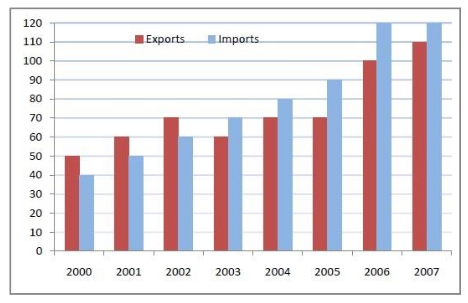
\includegraphics[width=0.6\linewidth]{figs/screenshot003}
				\caption{}
				\label{fig:screenshot003}
			\end{figure}
			
				
				\hfill{\brak{\text{GATE CS 2015}}}
				
				\item The head of a newly formed government desires to appoint five of the six selected members P,Q,R,S,T and U to portfolios of Home, Power, Defense, Telecom, and Finance. U does not want any portfolio if S gets one of the five. R wants either Home or Finance or no portfolio. Q says that if S gets either Power or Telecom, then she must get the other one. T insists on a portfolio if P gets one. Which is the valid distribution of portfolios?
				
				\hfill{\brak{\text{GATE CS 2015}}}
				
				\begin{enumerate}
					\begin{multicols}{2}
\item P-Home, Q-Power, R-Defense, S-Telecom, T-Finance
\item R-Home, S-Power, P-Defense, Q-Telecom, T-Finance
\item P-Home, Q-Power, T-Defense, S-Telecom, U-Finance
\item Q-Home, U-Power, T-Defense, R-Telecom, P-Finance
					\end{multicols}
					
				\end{enumerate}
				
				\item Choose the most appropriate equation for the function drawn as a thick line, in the plot below.
				
\begin{figure}[H]
	\centering
	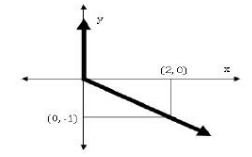
\includegraphics[width=0.4\linewidth]{figs/screenshot002}
\end{figure}

				
				\hfill{\brak{\text{GATE CS 2015}}}
				
				\begin{enumerate}
					\begin{multicols}{4}
					\item $x - y + y = 0$
					\item $-x + y + y = 0$
					\item $x + y - y = 0$
					\item $-x - y + y = 0$
				\end{multicols}
				
				\end{enumerate}
				
				\item Most experts feel that in spite of possessing all the technical skills required to be a batsman of the highest order, he is unlikely to be so due to lack of requisite temperament. He was guilty of throwing away his wicket several times after working hard to lay a strong foundation. His critics pointed out that until he addressed this problem success at the highest level will continue to elude him. Which of the statement\brak{\text{s}} below is/are logically valid and can be inferred from the above passage?
				\begin{align*}
					&\text{(i) He was already a successful batsman at the highest level}\\
					&\text{(ii) He has to improve his temperament in order to become a great batsman}\\
					&\text{(iii) He failed to make many of his good starts count}\\
					&\text{(iv) Improving his technical skills will guarantee success}
				\end{align*}
				
				\hfill{\brak{\text{GATE CS 2015}}}
				
				\begin{enumerate}
					\begin{multicols}{2}
						\item \brak{\text{iii}} and \brak{\text{iv}}
						\item \brak{\text{ii}} and \brak{\text{iii}}
						\item \brak{\text{i}}, \brak{\text{ii}} and \brak{\text{iii}}
						\item \brak{\text{ii}} only
					\end{multicols}
				\end{enumerate}
				
				\item Alexander turned his attention towards India, since he had conquered Persia. Which one of the statements below is logically valid and can inferred from the above sentence?
				
				\hfill{\brak{\text{GATE CS 2015}}}
				
				\begin{enumerate}
					\item Alexander would not have turned his attention towards India had he not conquered Persia.
					\item Alexander was not ready to rest on his laurels, and wanted to march to India
					\item Alexander was completely in control of his army and could command it to move towards India
					\item Since Alexander's kingdom extended to Indian borders after the conquest of Persia, he was keen to move further
				\end{enumerate}
				
			\end{enumerate}
			\newpage
			
			\section*{\Large COMPUTER SCIENCE AND INFORMATION TECHNOLOGY}
			\vspace{0.7cm}
			\fbox{\Large Q. No. 1 - 25 Carry One Mark Each}
						\vspace{0.7cm}
			\begin{enumerate}
				
				\item In a room there are only two types of people, namely Type $1$ and Type $2$. Type $1$ people always tell the truth and Type $2$ people always lie. You give a fair coin to a person in that room, without knowing which type he is from and tell him to Toss it and hide the result from you till you ask for it. Upon asking, the person replies the following. "The result of the toss is head if and only if I am telling the truth." Which of the following options is correct?
				
				\hfill{\brak{\text{GATE CS 2015}}}
				
				\begin{enumerate}
					\begin{multicols}{2}
						\item The result is head
						\item The result is tail
						\item If the person is of Type $2$, then the result is tail
						\item If the person is of Type $1$, then the result is tail
					\end{multicols}
				\end{enumerate}
				
				\item Consider the relation $X\brak{P,Q,R,S,T,U}$ with the following set of functional dependencies
				\begin{align*}
					F = \{\{P, R\} \rightarrow \{S,T\}, \{P,S, U\} \rightarrow \{Q, R\}\}
				\end{align*}
				Which of the following is the trivial functional dependency in $F^+$, where $F^+$ is closure of $F$?
				
				\hfill{\brak{\text{GATE CS 2015}}}
				
				\begin{enumerate}
					\begin{multicols}{2}
						\item $\{P,R\} \rightarrow \{S,T\}$
						\item $\{P,R\} \rightarrow \{R,T\}$
						\item $\{P,S\} \rightarrow \{S\}$
						\item $\{P,S,U\} \rightarrow \{Q\}$
					\end{multicols}
				\end{enumerate}
				
				\item Given a hash table $T$ with $25$ slots that stores $2000$ elements, the load factor $\alpha$ for $T$ is \underline{\hspace{2cm}}.
				
				\hfill{\brak{\text{GATE CS 2015}}}
				
				\item Consider a software project with the following information domain characteristics for calculation of function point metric.
				\begin{align*}
					&\text{Number of external inputs } (I) = 30\\
					&\text{Number of external outputs } (O) = 60\\
					&\text{Number of external inquiries } (E) = 23\\
					&\text{Number of files } (F) = 08\\
					&\text{Number of external interfaces } (N) = 02
				\end{align*}
				It is given that the complexity weighting factors for $I$, $O$, $E$, $F$ and $N$ are $4$,$5$,$4$,$10$ and $7$, respectively. It is also given that, out of fourteen value adjustment factors that influence the development effort, four factors are not applicable, each of the other four factors have value $3$, and each of the remaining factors have value $4$. The computed value of function point metric is \underline{\hspace{2cm}}.
				
				\hfill{\brak{\text{GATE CS 2015}}}
				
				\item Consider the following statements.
				\begin{align*}
					&\text{I. TCP connections are full duplex}\\
					&\text{II. TCP has no option for selective acknowledgment}\\
					&\text{III. TCP connections are message streams}
				\end{align*}
				
				\hfill{\brak{\text{GATE CS 2015}}}
				
				\begin{enumerate}
					\begin{multicols}{2}
						\item Only I is correct
						\item Only I and III are correct
						\item Only II and III are correct
						\item All of I, II and III are correct
					\end{multicols}
				\end{enumerate}
				
				\item Suppose $U$ is the power set of the set $S = \{1,2,3,4,5,6\}$. For any $T \subseteq U$, let $\abs{T}$ denote the number of element in $T$ and $T'$ denote the complement of $T$. For any $T,R \subseteq U$, let $T \setminus R$ be the set of all elements in $T$ which are not in $R$. Which one of the following is true?
				
				\hfill{\brak{\text{GATE CS 2015}}}
				
				\begin{enumerate}
					\item $\forall X \in U \colon \abs{X} = \abs{X'}$
					\item $\forall X \in U, \forall Y \in U \colon \abs{X} = 5, \abs{Y} = 5 \text{ and } X \neq Y$
					\item $\forall X \in U, \forall Y \in U \colon \abs{X} = 2, \abs{Y} = 3 \text{ and } \abs{X \setminus Y} = 2$
					\item $\forall X \in U, \forall Y \in U \colon \abs{X \setminus Y} = \abs{Y' \setminus X'}$
				\end{enumerate}
				
				\item Among simple LR \brak{\text{SLR}}, canonical LR, and look-ahead LR \brak{\text{LALR}}, which of the following pairs identify the method that is very easy to implement and the method that is the most powerful, in that order?
				
				\hfill{\brak{\text{GATE CS 2015}}}
				
				\begin{enumerate}
					\begin{multicols}{2}
						\item SLR, LALR
						\item Canonical LR, LALR
						\item SLR, canonical LR
						\item LALR, canonical LR
					\end{multicols}
				\end{enumerate}
				
				\item Consider the following array of elements.
				$$\langle 89,19,50,17,12,15,2,5,7,11,6,9,100 \rangle$$
				The minimum number of interchanges needed to convert it into a max-heap is
				
				\hfill{\brak{\text{GATE CS 2015}}}
				
				\begin{enumerate}
					\begin{multicols}{4}
						\item $4$
						\item $5$
						\item $2$
						\item $3$
					\end{multicols}
				\end{enumerate}
				
				\item The maximum number of processes that can be in Ready state for a computer system with $n$ CPUs is
				
				\hfill{\brak{\text{GATE CS 2015}}}
				
				\begin{enumerate}
					\begin{multicols}{4}
						\item $n$
						\item $n^2$
						\item $2^n$
						\item Independent of $n$
					\end{multicols}
				\end{enumerate}
				
				\item While inserting the elements $71,65,84,69,67,83$ in an empty binary search tree \brak{\text{BST}} in the sequence shown, the element in the lowest level is
				
				\hfill{\brak{\text{GATE CS 2015}}}
				
				\begin{enumerate}
					\begin{multicols}{4}
						\item $65$
						\item $67$
						\item $69$
						\item $83$
					\end{multicols}
				\end{enumerate}
				
				\item Two processes X and Y need to access a critical section. Consider the following synchronization construct used by both the processes.
				
				% CODE BLOCK showing Process X and Process Y synchronization
				
				\hfill{\brak{\text{GATE CS 2015}}}
				
				Here, $\text{varP}$ and $\text{varQ}$ are shared variables and both are initialized to false. Which one of the following statements is true?
				
				\begin{enumerate}
					\item The proposed solution prevents deadlock but fails to guarantee mutual exclusion
					\item The proposed solution guarantees mutual exclusion but fails to prevent deadlock
					\item The proposed solution guarantees mutual exclusion and prevents deadlock
					\item The proposed solution fails to prevent deadlock and fails to guarantee mutual exclusion
				\end{enumerate}
				
				\item Let \# be a binary operator defined as $X \# Y = X' + Y'$ where $X$ and $Y$ are Boolean variables. Consider the following two statements.
				\begin{align*}
					&\text{(S1) } (P\#Q)\#R = P\#(Q\#R)\\
					&\text{(S2) } Q\#R = R\#Q
				\end{align*}
				Which of the following is/are true for the Boolean variables $P$, $Q$ and $R$?
				
				\hfill{\brak{\text{GATE CS 2015}}}
				
				\begin{enumerate}
					\begin{multicols}{2}
						\item Only S1 is true
						\item Only S2 is true
						\item Both S1 and S2 are true
						\item Neither S1 nor S2 are true
					\end{multicols}
				\end{enumerate}
				
				\item Consider the following relation
				$$\text{Cinema } (\text{theater}, \text{address}, \text{capacity})$$
				Which of the following options will be needed at the end of the SQL query
				\begin{align*}
					&\text{SELECT P1. address}\\
					&\text{FROM Cinema P1}
				\end{align*}
				Such that it always finds the addresses of theaters with maximum capacity?
				
				\hfill{\brak{\text{GATE CS 2015}}}
				
				\begin{enumerate}
					\item WHERE P1. Capacity$>=$ All \brak{\text{select P2. Capacity from Cinema P2}}
					\item WHERE P1. Capacity$>=$ Any \brak{\text{select P2. Capacity from Cinema P2}}
					\item WHERE P1. Capacity$>=$ All \brak{\text{select max(P2. Capacity) from Cinema P2}}
					\item WHERE P1. Capacity$>=$ Any \brak{\text{select max (P2. Capacity) from Cinema P2}}
				\end{enumerate}
				
				\item The value of $\lim_{x \to \infty} \brak{1 - x} e^{2x}$ is
				
				\hfill{\brak{\text{GATE CS 2015}}}
				
				\begin{enumerate}
					\begin{multicols}{4}
						\item $0$
						\item $-\frac{1}{2}$
						\item $1$
						\item $\infty$
					\end{multicols}
				\end{enumerate}
				
				\item Consider the following C program segment.
				\begin{verbatim}
					#include <stdio.h>
					int main()
					{
						char s1[7] = "1234", *p;
						p = s1 + 2;
						*p = '0';
						printf("%s", s1);
					}
				\end{verbatim}
				What will be printed by the program?
				
				\hfill{\brak{\text{GATE CS 2015}}}
				
				\begin{enumerate}
					\begin{multicols}{4}
						\item $12$
						\item $120400$
						\item $1204$
						\item $1034$
					\end{multicols}
				\end{enumerate}
				
				\item The number of $4$ digit numbers having their digits in non-decreasing order \brak{\text{from left to right}} constructed by using the digits belonging to the set $\{1,2,3\}$ is \underline{\hspace{2cm}}.
				
				\hfill{\brak{\text{GATE CS 2015}}}
				
				\item In the matrix $\myvec{1 & 1 & 2 \\ 0 & 1 & 0 \\ 1 & 2 & 1}$, one of the eigen values is $1$. The eigen vectors corresponding to the eigen value $1$ are
				
				\hfill{\brak{\text{GATE CS 2015}}}
				
				\begin{enumerate}
					\begin{multicols}{2}
						\item $\alpha \brak{4,2,1}, \alpha \neq 0, \alpha \in \mathbb{R}$
						\item $\alpha \brak{-4,2,1}, \alpha \neq 0, \alpha \in \mathbb{R}$
						\item $\alpha \brak{-2,0,1}, \alpha \neq 0, \alpha \in \mathbb{R}$
						\item $\alpha \brak{2,0,1}, \alpha \neq 0, \alpha \in \mathbb{R}$
					\end{multicols}
				\end{enumerate}
				
				\item Consider a machine with byte addressable main memory of $2^{20}$ bytes, block size of $16$ bytes and a direct mapped cache having $2^{12}$ cache lines. Let the address of two consecutive bytes in main memory be $\brak{E201F}_{16}$ and $\brak{E2020}_{16}$. What are the tag and cache line address \brak{\text{in hex}} for main memory address $\brak{E201F}_{16}$?
				
				\hfill{\brak{\text{GATE CS 2015}}}
				
				\begin{enumerate}
					\begin{multicols}{4}
						\item E, $201$
						\item F, $201$
						\item E, E$20$
						\item $2$, $01$F
					\end{multicols}
				\end{enumerate}
				
				\item Consider the equality $\sum_{i=0}^{n} i^3 = X$ and the following choices for $X$
				\begin{align*}
					&\text{I. } O\brak{n^4}\\
					&\text{II. } O\brak{n^5}\\
					&\text{III. } O\brak{n^5}\\
					&\text{IV. } \Theta\brak{n^3}
				\end{align*}
				The equality above remains correct if $X$ is replaced by
				
				\hfill{\brak{\text{GATE CS 2015}}}
				
				\begin{enumerate}
					\begin{multicols}{2}
						\item Only I
						\item Only II
						\item I or III or IV but not II
						\item II or III or IV but not I
					\end{multicols}
				\end{enumerate}
				
				\item The result evaluating the postfix expression $10\ 5\ +\ 60\ 6\ /\ *\ 8\ -$ is
				
				\hfill{\brak{\text{GATE CS 2015}}}
				
				\begin{enumerate}
					\begin{multicols}{4}
						\item $284$
						\item $213$
						\item $142$
						\item $71$
					\end{multicols}
				\end{enumerate}
				
				\item Consider a CSMA/CD network that transmits data at a rate of $100$ Mbps \brak{10^8 \text{ bits per second}} over a $1$ km\brak{\text{kilometer}} cable with no repeaters. If the minimum frame size required for this network is $1250$ bytes, what is the signal speed \brak{\text{km/sec}} in the cable?
				
				\hfill{\brak{\text{GATE CS 2015}}}
				
				\begin{enumerate}
					\begin{multicols}{4}
						\item $8000$
						\item $10000$
						\item $16000$
						\item $20000$
					\end{multicols}
				\end{enumerate}
				
				\item Consider a software program that is artificially seeded with $100$ faults. While testing this program, $159$ faults are detected, out of which $75$ faults are from those artificially seeded faults. Assuming that both seeded and real faults are of same nature and have same distribution, the estimated number of undetected real fault is \underline{\hspace{2cm}}.
				
				\hfill{\brak{\text{GATE CS 2015}}}
				
				\item Consider a binary tree $T$ that has $200$ leaf nodes. Then, the number of nodes in $T$ that have exactly two children are \underline{\hspace{2cm}}.
				
				\hfill{\brak{\text{GATE CS 2015}}}
				
				\item In a web server, ten Web pages are stored with the URLs of the form http://www.yourname.com/var.html; where, var is different number from $1$ to $10$ for each Webpage. Suppose, the client stores the Webpage with var = $1$\brak{\text{say W1}} in local machine, edits and then tests. Rest of the Web pages remains on the web server. W1 contains several relative URLs of the form "var.html" referring to the other web pages. Which one of the following statements needs to be added in W1, so that all the relative URLs in W1 refers to the appropriate Web pages on the web server?
				
				\hfill{\brak{\text{GATE CS 2015}}}
				
				\begin{enumerate}
					\item $<$a href:"http://www.yourname.com/", href:"...var.html"$>$
					\item $<$base href:"http://www.yourname.com/"$>$
					\item $<$a href:"http://www.yourname.com/"$>$
					\item $<$base href:"http://www.yourname.com/", range:"...var.html"$>$
				\end{enumerate}
				
				\item Let $L$ be the language represented by the regular expression $\Sigma^*0011\Sigma^*$ where $\Sigma = \{0,1\}$. What is the minimum number of states in a DFA that recognizes $\overline{L}$ \brak{\text{complement of L}}?
				
				\hfill{\brak{\text{GATE CS 2015}}}
				
				\begin{enumerate}
					\begin{multicols}{4}
						\item $4$
						\item $5$
						\item $6$
						\item $8$
					\end{multicols}
				\end{enumerate}
				\fbox{\Large Q. No. 26 - 55 Carry Two Marks Each}
				
				\item If for non-zero $x$, $af\brak{\frac{1}{x}} + bf\brak{x} = \frac{25}{x}$ where $a \neq b$ then $\int_1^2 f(x)dx$ is
				
				\hfill{\brak{\text{GATE CS 2015}}}
				
				\begin{enumerate}
					\begin{multicols}{2}


					\item $\frac{a}{a^2 - b^2} \ln 2 + \frac{47b}{2\brak{a^2 - b^2}} \cdot \frac{1}{25}$
					\item $\frac{a}{a^2 - b^2} 2\ln 2 + \frac{47b}{2\brak{a^2 - b^2}} \cdot \frac{1}{25}$
					\item $\frac{a}{a^2 - b^2} 2\ln 2 - \frac{47b}{2\brak{a^2 - b^2}} \cdot \frac{1}{25}$
					\item $\frac{a}{a^2 - b^2} \ln 2 - \frac{47b}{2\brak{a^2 - b^2}} \cdot \frac{1}{25}$
										\end{multicols}
				\end{enumerate}
				
				\item Consider the following grammar $G$
				\begin{align*}
					S &\rightarrow F | H\\
					S &\rightarrow p | c\\
					S &\rightarrow d | c
				\end{align*}
				where $S$, $F$, and $H$ are non-terminal symbols, $p$, $d$, and $c$ are terminal symbols. Which of the following statements\brak{\text{s}} is/are correct?
				\begin{align*}
					&\text{S1: LL(1) can parse all strings that are generated using grammar G}\\
					&\text{S2: LR(1) can parse all strings that are generated using grammar G}
				\end{align*}
				
				\hfill{\brak{\text{GATE CS 2015}}}
				
				\begin{enumerate}
					\begin{multicols}{4}
						\item Only S1
						\item Only S2
						\item Both S1 and S2
						\item Neither S1 nor S2
					\end{multicols}
				\end{enumerate}
				
				\item Consider three software items: Program –X, Control Flow Diagram of Program-Y and Control Flow Diagram of Program –Z as shown below
				
				\begin{figure}[H]
					\centering
					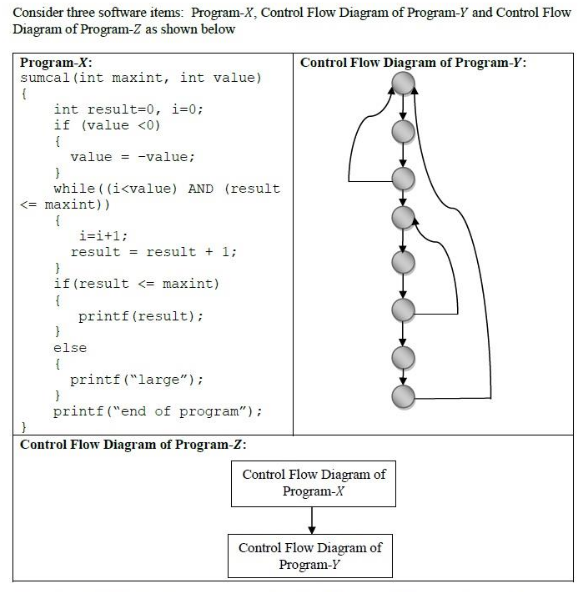
\includegraphics[width=0.7\linewidth]{figs/screenshot001}
				\end{figure}
				
				
				\hfill{\brak{\text{GATE CS 2015}}}
				
				The values of McCabe's Cyclomatic complexity of Program –X, Program-Y, and Program-Z respectively are
				
				\begin{enumerate}
					\begin{multicols}{4}
						\item $4, 4, 7$
						\item $3, 4, 7$
						\item $4, 4, 8$
						\item $4, 3, 8$
					\end{multicols}
				\end{enumerate}
				
				\item Consider the following partial Schedule $S$ involving two transactions $T1$ and $T2$. Only the read and write operations have been shown. The read operation on data item $P$ is denoted by read\brak{P} and the write operation on data item $P$ is denoted by write\brak{P}.
				
				\begin{table}[h]
					\centering
					\caption*{}
					\label{tab:schedule}
					\begin{tabular}{|c|c|c|}
						\hline
						Time instance & \multicolumn{2}{c|}{Transaction-id} \\
						\cline{2-3}
						& T1 & T2 \\
						\hline
						1 & read(A) & \\
												\hline
						2 & write(A) & \\
												\hline
						3 & read(C) & \\
												\hline
												
						4 & write(C) & \\
												\hline
						5 & read(B) & \\
												\hline
						6 & write(B) & \\
												\hline
						7 & & read(A) \\
												\hline
						8 & & commit \\
												\hline
						9 & read(B) & \\
						\hline
					\end{tabular}
				\end{table}
				
				Suppose that the transaction $T1$ fails immediately after time instance $9$. Which one of the following statements is correct?
				
				\hfill{\brak{\text{GATE CS 2015}}}
				
				\begin{enumerate}
					\item $T2$ must be aborted and then both $T1$ and $T2$ must be re-started to ensure transaction atomicity
					\item Schedule $S$ is non-recoverable and cannot ensure transaction atomicity
					\item Only $T2$ must be aborted and then re-started to ensure transaction atomicity
					\item Schedule $S$ is recoverable and can ensure atomicity and nothing else needs to be done
				\end{enumerate}
				
				\item Consider a B+ tree in which the search key is $12$ bytes long, block size is $1024$ bytes, record pointer is $10$ bytes long and block pointer is $8$ bytes long. The maximum number of keys that can be accommodated in each non-leaf node of the tree is \underline{\hspace{2cm}}.
				
				\hfill{\brak{\text{GATE CS 2015}}}
				
				\item Suppose $X_i$ for $i=1,2,3$ are independent and identically distributed random variables whose probability mass functions are
				$$P_r\brak{X_i = 0} = P_r\brak{X_i = 1} = 1/2 \text{ for } i = 1,2,3.$$
				Define another random variable $Y = X_1 \oplus X_2 \oplus X_3$, where $\oplus$ denotes XOR. Then $P_r\brak{Y = 0 | X_3 = 0}$ = \underline{\hspace{2cm}}.
				
				\hfill{\brak{\text{GATE CS 2015}}}
				
				\item Given the function $F = P + QR$, where $F$ is a function in three Boolean variables $P$, $Q$ and $R$ and $P = !P$, consider the following statements
				\begin{align*}
					&\text{(S1) } F \in \{4,5,6\}\\
					&\text{(S2) } F \in \{0,1,2,3,7\}\\
					&\text{(S3) } F' \in \{4,5,6\}\\
					&\text{(S4) } F' \in \{0,1,2,3,7\}
				\end{align*}
				Which of the following is true?
				
				\hfill{\brak{\text{GATE CS 2015}}}
				
				\begin{enumerate}
					\begin{multicols}{2}


					\item \brak{\text{S1}}-False, \brak{\text{S2}}-True, \brak{\text{S3}}-True, \brak{\text{S4}}-False
					\item \brak{\text{S1}}-True, \brak{\text{S2}}-False, \brak{\text{S3}}-False, \brak{\text{S4}}-True
					\item \brak{\text{S1}}-False, \brak{\text{S2}}-False, \brak{\text{S3}}-True, \brak{\text{S4}}-True
					\item \brak{\text{S1}}-True, \brak{\text{S2}}-True, \brak{\text{S3}}-False, \brak{\text{S4}}-False
										\end{multicols}
				\end{enumerate}
				
				\item The total number of prime implicates of the function $f\brak{w,x,y,z} = \sum\brak{0,2,4,5,6,10}$ is \underline{\hspace{2cm}}.
				
				\hfill{\brak{\text{GATE CS 2015}}}
				
				\item Consider the equation $\brak{43}_x = \brak{y3}_8 $ where $x$ and $y$ are unknown. The number of possible solutions is \underline{\hspace{2cm}}.
				
				\hfill{\brak{\text{GATE CS 2015}}}
				
				\item Let $f(n)=n$ and $g(n)=n^{1+\sin n}$, where $n$ is a positive integer. Which of the following statement is/are correct?
				\begin{align*}
					&\text{I. } f(n) = O\brak{g(n)}\\
					&\text{II. } f(n) = \Omega\brak{g(n)}
				\end{align*}
				
				\hfill{\brak{\text{GATE CS 2015}}}
				
				\begin{enumerate}
					\begin{multicols}{4}
						\item Only I
						\item Only II
						\item Both I and II
						\item Neither I nor II
					\end{multicols}
				\end{enumerate}
				
				\item Suppose $c = \brak{c_0, c_1, \ldots, c_{k-1}}$ is an array of length $k$, where all the entries are from the set $\{0, 1\}$. For any positive integers $a$ and $n$, consider the following pseudo code.
				\begin{verbatim}
					DOSOMETHING (c, a, n)
					z = 1
					for i = 0 to k-1
					do z = z^2 mod n
					if c[i] = 1
					then z = z * a mod n
					return z
				\end{verbatim}
				If $k = 4$, $c = \brak{1,0,1,1}$, $a = 2$ and $n = 8$, then the output of DOSOMETHING \brak{c, a, n} is \underline{\hspace{2cm}}.
				
				\hfill{\brak{\text{GATE CS 2015}}}
				
				\item Consider the following recursive C function.
				\begin{verbatim}
					void get (int n)
					{
						if (n < 1) return;
						get (n-1);
						get (n-3);
						printf (" %d", n);
					}
				\end{verbatim}
				If get \brak{6} function is being called in main \brak{} then how many times will the get \brak{} function be invoked before returning to the main \brak{}?
				
				\hfill{\brak{\text{GATE CS 2015}}}
				
				\begin{enumerate}
					\begin{multicols}{4}
						\item $15$
						\item $25$
						\item $35$
						\item $45$
					\end{multicols}
				\end{enumerate}
				
				\item Assume that a mergesort algorithm in the worst case takes $30$ second for an input of size $64$. Which of the following most closely approximates the maximum input size of a problem that can be solved in $6$ minutes?
				
				\hfill{\brak{\text{GATE CS 2015}}}
				
				\begin{enumerate}
					\begin{multicols}{4}
						\item $256$
						\item $512$
						\item $1024$
						\item $2048$
					\end{multicols}
				\end{enumerate}
				
				\item Consider the following two C code segments. $Y$ and $X$ are one and two dimensional arrays of size $n$ and $n \times n$ respectively, where $2 \leq n \leq 10$. Assume that in both code segments, elements of $Y$ are initialized to $0$ and each element $X[i][j]$ of array $X$ is initialized to $i + j$. Further assume that when stored in main memory all elements of $X$ are in same main memory page frame.
				
				Code segment $1$:
				\begin{verbatim}
					//initialize element of Y to 0
					//initialize elements X[i][j] of X to i+j
					For (i = 0; i < n; i++)
					Y[i] += x[0][i];
				\end{verbatim}
				
				Code segment $2$:
				\begin{verbatim}
					//initialize elements of Y to 0
					//initialize elements X[i][j] of X to i+j
					For (i = 0; i < n; i++)
					Y[i] += x[i][0];
				\end{verbatim}
				
				Which of the following statements is/are correct?
				\begin{align*}
					&\text{S1: Final contents of array Y will be same in both code segments}\\
					&\text{S2: Elements of array X accessed inside the for loop shown in code segment 1 are contiguous in main memory}\\
					&\text{S3: Elements of array X accessed inside the for loop shown in code segment 2 are contiguous in main memory.}
				\end{align*}
				
				\hfill{\brak{\text{GATE CS 2015}}}
				
				\begin{enumerate}
					\begin{multicols}{2}
						\item Only S2 is correct
						\item Only S3 is correct
						\item Only S1 and S2 are correct
						\item Only S1 and S3 are correct
					\end{multicols}
				\end{enumerate}
				
				\item The velocity $v$ \brak{\text{in kilometer/minute}} of a motorbike which starts from rest, is given at fixed intervals of time $t$ \brak{\text{in minutes}} as follows.
				
				\begin{table}[h]
					\centering
					\caption*{}
					\label{tab:velocity}
					\begin{tabular}{|c|c|c|c|c|c|c|c|c|c|c|}
						\hline
						$t$ & $2$ & $4$ & $6$ & $8$ & $10$ & $12$ & $14$ & $16$ & $18$ & $20$ \\
						\hline
						$v$ & $10$ & $18$ & $25$ & $29$ & $32$ & $20$ & $11$ & $5$ & $2$ & $0$ \\
						\hline
					\end{tabular}
				\end{table}
				
				The approximate distance \brak{\text{in kilometers}} rounded to two places of decimals covered in $20$ minutes using Simpson's $1/3^{rd}$ rule is \underline{\hspace{2cm}}.
				
				\hfill{\brak{\text{GATE CS 2015}}}
				
				\item Consider the following C program
				\begin{verbatim}
					#include <stdio.h>
					int main()
					{
						static int a[] = {10,20,30,40,50};
						static int *p[] = {a,a+3,a+4,a+1,a+2};
						int **ptr = p;
						ptr++;
						printf("%d%d", ptr-p,**ptr);
					}
				\end{verbatim}
				The output of the program is \underline{\hspace{2cm}}.
				
				\hfill{\brak{\text{GATE CS 2015}}}
				
				\item Consider the following policies for preventing deadlock in a system with mutually exclusive resources.
				\begin{align*}
					&\text{I. Processes should acquire all their resources at the beginning of execution. If any resources}\\
					&\quad \text{cannot be acquired, then all resources acquired so far are released.}\\
					&\text{II. The resources are numbered uniquely, and processes are allowed to request for resources only}\\
					&\quad \text{in increasing resource numbers.}\\
					&\text{III. The resources are numbered uniquely, and processes are allowed to request for resources only}\\
					&\quad \text{in decreasing resource numbers.}\\
					&\text{IV. The resources are numbered uniquely. A process is allowed to request only for a resource with}\\
					&\quad \text{resource number larger than its currently held resources.}
				\end{align*}
				Which of the above policies can be used for preventing deadlock?
				
				\hfill{\brak{\text{GATE CS 2015}}}
				
				\begin{enumerate}
					\begin{multicols}{2}
						\item Any one of I and III but not II or IV
						\item Any one of I, III, and IV but not II
						\item Any one of II and III but not I or IV
						\item Any one of I, II, III, and IV
					\end{multicols}
				\end{enumerate}
				
				\item Let $G$ be a connected undirected graph of $100$ vertices and $300$ edges. The weight of a minimum spanning tree of $G$ is $500$. When the weight of each edge of $G$ is increased by five, the weight of a minimum spanning tree becomes \underline{\hspace{2cm}}.
				
				\hfill{\brak{\text{GATE CS 2015}}}
				
				\item If the following system has non-trivial solution.
				\begin{align*}
					px + qy + rz &= 0\\
					qx + ry + pz &= 0\\
					rx + py + qz &= 0
				\end{align*}
				Then which one of the following options is TRUE?
				
				\hfill{\brak{\text{GATE CS 2015}}}
				
				\begin{enumerate}
					\begin{multicols}{2}
\item $p + q + r = 0$ or $p = q = r$
\item $p + q + r = 0$ or $p = q = -r$
\item $p + q + r = 0$ or $p = q = r$
\item $p + q + r = 0$ or $p = -q = r$
					\end{multicols}
					
				\end{enumerate}
				
				\item Consider a network connecting two systems located $8000$ kilometers apart. The bandwidth of the network is $500 \times 10^6$ bits per second. The propagation speed of the media is $4 \times 10^6$ meters per second. It is needed to design a Go-Back-N sliding window protocol for this network. The average packet size is $10^7$ bits. The network is to be used to its full capacity. Assume that processing delays at nodes are negligible. Then the minimum size in bits of the sequence number field has to be \underline{\hspace{2cm}}.
				
				\hfill{\brak{\text{GATE CS 2015}}}
				
				\item Language $L_1$ is polynomial time reducible to language $L_2$. Language $L_3$ is polynomial time reducible to $L_2$, which in turn is polynomial time reducible to language $L_4$. Which of the following is/are true?
				\begin{align*}
					&\text{I. if } L_4 \in P, \text{ then } L_2 \in P\\
					&\text{II. if } L_1 \in P \text{ or } L_3 \in P, \text{ then } L_2 \in P\\
					&\text{III. } L_1 \in P, \text{ if and only if } L_3 \in P\\
					&\text{IV. if } L_4 \in P, \text{ then } L_1 \in P \text{ and } L_3 \in P
				\end{align*}
				
				\hfill{\brak{\text{GATE CS 2015}}}
				
				\begin{enumerate}
					\begin{multicols}{4}
						\item II only
						\item III only
						\item I and IV only
						\item I only
					\end{multicols}
				\end{enumerate}
				
				\item Consider the following reservation table for a pipeline having three stages $S_1$, $S_2$, and $S_3$.
				
				\begin{table}[h]
					\centering
					\caption*{}
					\label{tab:reservation}
					\begin{tabular}{|c|c|c|c|c|c|}
						\hline
						& \multicolumn{5}{c|}{Time} \\
						\cline{2-6}
						& $1$ & $2$ & $3$ & $4$ & $5$ \\
						\hline
						$S_1$ & X & &   & & X \\
						\hline
						$S_2$ & & X & & X & \\
						\hline
						$S_3$ & & & X & & \\
						\hline
					\end{tabular}
				\end{table}
				
				The minimum average latency \brak{\text{MAL}} is \underline{\hspace{2cm}}.
				
				\hfill{\brak{\text{GATE CS 2015}}}
				
				\item In the network $200.20.11.144/27$, the fourth octet \brak{\text{in decimal}} of the last IP address of the network which can be assigned to a host is \underline{\hspace{2cm}}.
				
				\hfill{\brak{\text{GATE CS 2015}}}
				
				\item Which of the following languages are context-free?
				\begin{align*}
					L_1 &= \{a^m b^n a^n b^m \mid m, n \geq 1\}\\
					L_2 &= \{a^m b^n a^m b^n \mid m, n \geq 1\}\\
					L_3 &= \{a^m b^n \mid m = 2n + 1\}
				\end{align*}
				
				\hfill{\brak{\text{GATE CS 2015}}}
				
				\begin{enumerate}
					\begin{multicols}{4}
						\item $L_1$ and $L_2$ only
						\item $L_1$ and $L_3$ only
						\item $L_2$ and $L_3$ only
						\item $L_3$ only
					\end{multicols}
				\end{enumerate}
				
				\item Consider the following C program
				\begin{verbatim}
					#include <stdio.h>
					int main()
					{
						int i,j,k = 0;
						j= 2*3/4+ 2.0/5+8/5;
						k-= --j;
						for(i = 0;i < 5;i++)
						{
							switch(i + k)
							{
								case 1:
								case 2: printf("\n%d",i+ k);
								case 3: printf("\n%d",i+ k);
								default: printf("\n%d",i+ k);
							}
						}
						return 0;
					}
				\end{verbatim}
				The number of times printf statement is executed is \underline{\hspace{2cm}}.
				
				\hfill{\brak{\text{GATE CS 2015}}}
				
				\item Consider the following C program.
				\begin{verbatim}
					#include <stdio.h>
					int f1(void);
					int f2(void);
					int f3(void);
					int x = 10;
					int main()
					{
						int x = 1;
						x+= f1() + f2() + f3() + f2();
						printf("%d",x);
						return 0;
					}
					int f1() {int x = 25;x++;return x;}
					int f2() {static int x = 50;x++;return x;}
					int f3() {x*= 10;return x;}
				\end{verbatim}
				The output of the program is \underline{\hspace{2cm}}.
				
				\hfill{\brak{\text{GATE CS 2015}}}
				
				\item Consider the following code sequence having five instructions $I_1$ to $I_5$. Each of these instructions has the following format.
				$\text{OP } R_i, R_j, R_k$
				Where operation OP is performed on contents of registers $R_j$ and $R_k$ and the results is stored in register $R_i$.
				\begin{align*}
					I_1 &\colon \text{ADD } R_1, R_2, R_3\\
					I_2 &\colon \text{MUL } R_7, R_1, R_3\\
					I_3 &\colon \text{SUB } R_4, R_1, R_5\\
					I_4 &\colon \text{ADD } R_3, R_2, R_4\\
					I_5 &\colon \text{MUL } R_7, R_8, R_9
				\end{align*}
				Consider the following three statements.
				\begin{align*}
					&\text{S1: There is an anti-dependence between instructions } I_2 \text{ and } I_5\\
					&\text{S2: There is an anti-dependence between instructions } I_2 \text{ and } I_4\\
					&\text{S3: Within an instruction pipeline an anti-dependence always creates one or more stalls}
				\end{align*}
				Which one of above statements is/are correct?
				
				\hfill{\brak{\text{GATE CS 2015}}}
				
				\begin{enumerate}
					\begin{multicols}{2}
						\item Only S1 is true
						\item Only S2 is true
						\item Only S1 and S3 are true
						\item Only S2 and S3 are true
					\end{multicols}
				\end{enumerate}
				
				\item Two hosts are connected via a packet switch with $10^7$ bits per second links. Each link has a propagation delay of $20$ microseconds. The switch begins forwarding a packet $35$ microseconds after it receives the same. If $10000$ bits of data are to be transmitted between the two hosts using a packet size of $5000$ bits, the time elapsed between the transmission of the first bit of data and the reception of the last bit of the data in microseconds is \underline{\hspace{2cm}}.
				
				\hfill{\brak{\text{GATE CS 2015}}}
				
				\item Let $R$ be a relation on the set of ordered pairs of positive integers such that $\brak{(p,q), (r,s)} \in R$ if and only if $p + s = q + r$. Which one of the following is true about $R$?
				
				\hfill{\brak{\text{GATE CS 2015}}}
				
				\begin{enumerate}
					\begin{multicols}{2}
						\item Both reflexive and symmetric
						\item Reflexive but not symmetric
						\item Not reflexive but symmetric
						\item Neither reflexive nor symmetric
					\end{multicols}
				\end{enumerate}
				
				\item For the processes listed in the following table, which of the following scheduling schemes will give the lowest average turnaround time?
				
				\begin{table}[h]
					\centering
					\caption*{}
					\label{tab:processes}
					\begin{tabular}{|c|c|c|}
						\hline
						Process & Arrival Time & Processing Time \\
						\hline
						A & $0$ & $3$ \\
						B & $1$ & $6$ \\
						C & $4$ & $4$ \\
						D & $6$ & $2$ \\
						\hline
					\end{tabular}
				\end{table}
				
				\hfill{\brak{\text{GATE CS 2015}}}
				
				\begin{enumerate}
					\begin{multicols}{2}
\item First Come First Serve
\item Non-preemptive Shortest Job First
\item Shortest Remaining Time
\item Round Robin with Quantum value two
					\end{multicols}
					
				\end{enumerate}
				
			\end{enumerate}
			

		

\end{document}